\documentclass[12pt, letterpaper]{article}
\usepackage[utf8]{inputenc} % Input encoding
\usepackage[T1]{fontenc} % Font encoding
\usepackage{amsmath} % Math symbols and environments
\usepackage{amssymb} % More math symbols
\usepackage{graphicx} % Include graphics
\usepackage[spanish]{babel} % Spanish language support (ACTIVADO)
\usepackage{tabularx}
\usepackage{enumitem}
\renewcommand{\arraystretch}{1.5} % Incrementa el espaciado vertical
\graphicspath{ {./images/}} 

\begin{document}
\begin{titlepage}
    \centering
    % NOTA: He asumido que 'IN.png' es el logo correcto.
    
\includegraphics[width=2cm]{IN}\\[2cm] 
    \textsc{\LARGE  Instituto Nacional General José Miguel Carrera}\\[0.5cm]
    \textsc{\Large Departamento de Matemáticas}\\[1.5cm] % Corregido: Matemáticas
    
    \rule{\textwidth}{1.5pt}\vspace{0.4cm}
    {\Huge \bfseries Apunte Completo: \\[0.5cm] Probabilidad y Estadística}\\[0.4cm] % Corregido: Estadística
    \rule{\textwidth}{1.5pt}\\[1.5cm]
    
    {\Large \textit{ Probabilidad y Estadística - Sección 2025}}\\[2cm] % Corregido: Estadística
    
    \begin{minipage}{0.45\textwidth}
        \begin{flushleft} \large
            \textbf{Autor:}\\ 
            Felipe Colli Olea
        \end{flushleft}
    \end{minipage}
    \hfill
    \begin{minipage}{0.45\textwidth}
        \begin{flushright} \large
            \textbf{Profesor:}\\
            Sergio Díaz
        \end{flushright}
    \end{minipage}

    \vfill
    
    {\large 2 de julio de 2025}
\end{titlepage}

\begin{abstract}
    \noindent \textbf{Resumen} \\
    Este apunte ofrece una introducción completa a los conceptos fundamentales de la probabilidad y la estadística. Comienza con la definición de términos esenciales como población, muestra, parámetro y estadígrafo, y la clasificación de variables en cualitativas y cuantitativas. Posteriormente, se profundiza en la estadística descriptiva, abordando las medidas de tendencia central (media, mediana, moda) y de dispersión (rango, varianza, desviación estándar), incluyendo sus propiedades y demostraciones matemáticas. El documento también explora diversas técnicas de muestreo, diferenciando entre métodos probabilísticos (aleatorio simple, estratificado, por conglomerados, sistemático) y no probabilísticos. Finalmente, se introduce la combinatoria mediante los principios aditivo y multiplicativo como base para el cálculo de probabilidades.
\end{abstract}

\begin{figure}[htbp]
    \centering
    
\includegraphics[width=0.55\textwidth]{gatito}
    \caption{Gatito para hacer bonito el apunte.}
    \label{fig:gatito}
\end{figure}
\newpage

\tableofcontents
\newpage % Start sections on a new page after ToC

\section{14/03 - Conceptos Fundamentales de Estadística}
\subsection{Materia}
\textbf{Población:} % Simplificado el énfasis
Conjunto de todos los elementos que se quieren estudiar. Cuando la información deseada está disponible para todos los objetos de la población, lo llamamos \textbf{censo}. En la práctica es muy difícil o casi imposible realizar un censo.

\textbf{Muestra:} % Simplificado el énfasis
Subconjunto de la población que se mide u observa.

\textbf{Parámetro:} % Simplificado el énfasis
Es una medición numérica que describe alguna característica de una población.

\textbf{Estadístico (o estadígrafo):} % Simplificado el énfasis, añadido "o"
Es una medición numérica que describe alguna característica de la muestra.

\textbf{Variables cualitativas:} % Simplificado el énfasis
\begin{itemize}
    \item Se describen mediante palabras o categorías.
    \item Se usan para categorizar a los individuos o para identificar.
    \item Sirven para comprender aspectos subjetivos y complejos.
    \item Se pueden clasificar en nominales y ordinales.
    \item Ejemplos: el color del cabello, el deporte favorito, la comida favorita, el lugar de nacimiento.
\end{itemize}

\textbf{Variables cuantitativas:} % Simplificado el énfasis
\begin{itemize}
    \item Se expresan mediante números, es decir, se pueden contar o medir.
    \item Permiten más operaciones matemáticas.
    \item Se pueden usar para conocer fenómenos o situaciones a través de la recolección y generación de números y datos.
    \item Ejemplos: la edad, los ingresos, el peso, la altura, la presión, la humedad o cantidad de hermanos.
\end{itemize}

\subsection{Ejercicios:}
Para cada una de las siguientes situaciones, identifica la población de interés, la variable estadística, clasifícala, y entrega un ejemplo de cuál podría ser una posible muestra.

\begin{enumerate}
    \item Un investigador universitario desea estimar la proporción de ciudadanos chilenos de la \textit{GEN X} que están interesados en iniciar sus propios negocios.
        \begin{enumerate}
            \item \textbf{Población:} Chilenos de la Generación X.
            \item \textbf{Muestra (ejemplo):} 500 chilenos de la Generación X seleccionados aleatoriamente del padrón electoral.
            \item \textbf{Variable:} Interés en iniciar un negocio (Sí/No) (\textit{cualitativa nominal}).
        \end{enumerate}

    \item Durante más de un siglo, la temperatura corporal normal en seres humanos ha sido aceptada como 37°C. ¿Es así realmente? Los investigadores desean estimar el promedio de temperatura de adultos sanos en Chile.
        \begin{enumerate}
            \item \textbf{Población:} Adultos sanos en Chile.
            \item \textbf{Muestra (ejemplo):} Adultos sanos de Santiago seleccionados de diversos centros de salud.
            \item \textbf{Variable:} Temperatura corporal (\textit{cuantitativa continua}).
        \end{enumerate}

    \item Un ingeniero municipal desea estimar el promedio de consumo semanal de agua para unidades habitacionales unifamiliares en la ciudad.
        \begin{enumerate}
            \item \textbf{Población:} Unidades habitacionales unifamiliares de la ciudad.
            \item \textbf{Muestra (ejemplo):} 200 unidades habitacionales unifamiliares de distintos barrios de la ciudad, seleccionadas aleatoriamente.
            \item \textbf{Variable:} Consumo semanal de agua (en litros) (\textit{cuantitativa continua}).
        \end{enumerate}
    \item El National Highway Safety Council desea estimar la proporción de llantas para automóvil con dibujo o superficie de rodadura insegura, entre todas las llantas manufacturadas por una empresa específica durante el presente año de producción.
        \begin{enumerate}
            \item \textbf{Población:} Todas las llantas para automóvil manufacturadas por la empresa específica durante el presente año de producción.
            \item \textbf{Muestra (ejemplo):} Una selección aleatoria de llantas producidas en diferentes lotes o días del año.
            \item \textbf{Variable:} Estado de la superficie de rodadura (segura/insegura) (\textit{cualitativa nominal}).
        \end{enumerate}
    \item Un politólogo desea estimar si la mayoría de los residentes adultos de una región están a favor de una legislatura unicameral.
        \begin{enumerate}
            \item \textbf{Población:} Residentes adultos de la región.
            \item \textbf{Muestra (ejemplo):} Residentes adultos de varias comunas seleccionadas aleatoriamente de la región.
            \item \textbf{Variable:} Opinión sobre la legislatura unicameral (a favor/en contra/indeciso) (\textit{cualitativa nominal}).
        \end{enumerate}
    \item Un científico del área médica desea determinar el tiempo promedio para que se vuelva a presentar cierta enfermedad infecciosa, una vez que las personas se recuperan de ella por primera vez.
        \begin{enumerate}
            \item \textbf{Población:} Personas que se han recuperado de la enfermedad infecciosa por primera vez.
            \item \textbf{Muestra (ejemplo):} Pacientes recuperados seleccionados de registros médicos de diversos hospitales.
            \item \textbf{Variable:} Tiempo hasta la recurrencia de la enfermedad (\textit{cuantitativa continua}).
        \end{enumerate}
    \item Un ingeniero electricista desea determinar si el promedio de vida útil de transistores de cierto tipo es mayor que 500 horas.
        \begin{enumerate}
            \item \textbf{Población:} Todos los transistores de cierto tipo.
            \item \textbf{Muestra (ejemplo):} Una muestra de 100 transistores de ese tipo, seleccionados aleatoriamente de la producción.
            \item \textbf{Variable:} Vida útil del transistor (en horas) (\textit{cuantitativa continua}).
        \end{enumerate}
\end{enumerate}
\newpage

\section{17/03 - Tablas de Frecuencia y Medidas de Tendencia Central}
\subsection{Materia}
Medidas de Tendencia Central \\
Medidas de Posición \\
Medidas de Dispersión 

\textbf{Tablas de Frecuencia: Conceptos Básicos}
\begin{itemize}
    \item \textbf{Dato o Intervalo:} Información (variable) que se estudia en estadística.
    \item \textbf{Marca de Clase ($c_i$):} Promedio entre los extremos de un intervalo.
    \item \textbf{Amplitud de un intervalo:} Es la diferencia entre el límite superior y el límite inferior del intervalo.
\end{itemize}

\textbf{Tipos de Frecuencia:}
\begin{itemize}
    \item \textbf{Frecuencia Absoluta ($f_i$):} Cantidad de veces que se repite un dato o que los datos caen en un intervalo.
    \item \textbf{Frecuencia Absoluta Acumulada ($F_i$):} Suma de las frecuencias absolutas hasta determinado dato o intervalo. $F_i = \sum_{j=1}^{i} f_j$.
    \item \textbf{Frecuencia Relativa ($h_i$ o $f_{ri}$):} Es la proporción (fracción, decimal o porcentaje) de observaciones que corresponden a cierto valor o intervalo. ($h_i = \frac{f_i}{n}$), donde $n$ es el número total de datos.
    \item \textbf{Frecuencia Relativa Acumulada ($H_i$):} Es la proporción (fracción, decimal o porcentaje) de la frecuencia acumulada hasta cierto dato o intervalo. ($H_i = \frac{F_i}{n} = \sum_{j=1}^{i} h_j$).
\end{itemize}
\newpage

\textbf{Medidas de Tendencia Central:}
\begin{itemize}
    \item \textbf{Media Aritmética ($\bar{x}$):} Es el cociente entre la suma de todos los datos y el número total de datos ($n$). Si se tienen $n$ datos $x_1, x_2, \dots, x_n$:
        \[ \bar{x}=\frac{x_1+x_2+\dots+x_n}{n} = \frac{\sum_{i=1}^{n} x_i}{n} \] \\
    Para datos agrupados en una tabla de frecuencia con $k$ clases:
    % NOTA: Se ajustó el layout con minipage para evitar el Overfull hbox.
    \begin{center}
        \begin{minipage}{0.35\textwidth}
            \centering
            \begin{tabular}{|c|c|} 
                \hline
                \textbf{Marca ($c_i$)} & \textbf{Frec. ($f_i$)} \\
                \hline
                $c_1$ & $f_1$ \\
                \hline
                $c_2$ & $f_2$ \\
                \hline
                $\vdots$ & $\vdots$ \\
                \hline
                $c_k$ & $f_k$ \\
                \hline
             \end{tabular}
        \end{minipage}
        \hfill
        \begin{minipage}{0.55\textwidth}
            \centering
            \[ \bar{x}=\frac{c_1 f_1 + c_2 f_2 + \dots + c_k f_k}{f_1+f_2+\dots+f_k} = \frac{\sum_{i=1}^{k} c_i f_i}{n} \]
            (donde $n = \sum_{i=1}^{k} f_i$)
        \end{minipage}
    \end{center}

    \item \textbf{Mediana ($M_e$):} Es el valor que ocupa la posición central de la muestra cuando los datos se encuentran ordenados. \textbf{Si la muestra tiene un número par de datos, la mediana es la media aritmética de los dos términos centrales.}
        \begin{itemize}
            \item Si $n$ es impar, la posición es $\frac{n+1}{2}$. $M_e = x_{(\frac{n+1}{2})}$.
            \item Si $n$ es par, las posiciones son $\frac{n}{2}$ y $\frac{n}{2}+1$. $M_e = \frac{x_{(\frac{n}{2})} + x_{(\frac{n}{2}+1)}}{2}$.
        \end{itemize}
    \item \textbf{Moda ($M_o$):} Es el dato o intervalo con la mayor frecuencia absoluta. La muestra puede ser:
        \begin{itemize}
            \item \textbf{Amodal:} No presenta moda.
            \item \textbf{Unimodal:} Una sola moda.
            \item \textbf{Bimodal:} Dos modas.
            \item \textbf{Polimodal (o Multimodal):} Más de dos modas.
        \end{itemize}
\end{itemize}
\newpage

\section{26/03 - Ejercicios de Medidas de Tendencia Central}
\subsection{Ejercicios:}

\noindent % Evita la sangría
Si las notas de Esteban en una asignatura son \(3, 4, 6, 3, 5, 5, 6, 3, 4\) y de estas notas se cambian un $6$ por un $7$. ¿Cuál(es) de las siguientes medidas de tendencia central cambia(n)?
\begin{enumerate}
    \item La moda
    \item La mediana
    \item La media aritmética
\end{enumerate}
\textit{Solución:}
Notas originales (ordenadas): \(3, 3, 3, 4, 4, 5, 5, 6, 6\). $n=9$.
\begin{itemize}
    \item Moda original: 3 (frecuencia 3).
    \item Mediana original: El dato en la posición $\frac{9+1}{2}=5$. Mediana = 4.
    \item Media original: $\frac{3 \cdot 3 + 2 \cdot 4 + 2 \cdot 5 + 2 \cdot 6}{9} = \frac{39}{9} \approx 4.33$.
\end{itemize}
Notas nuevas (se cambia un 6 por un 7), ordenadas: \(3, 3, 3, 4, 4, 5, 5, 6, 7\). $n=9$.
\begin{itemize}
    \item Moda nueva: 3 (sigue siendo la más frecuente). $\rightarrow$ No cambia.
    \item Mediana nueva: El dato en la posición 5 sigue siendo 4. $\rightarrow$ No cambia.
    \item Media nueva: $\frac{39 - 6 + 7}{9} = \frac{40}{9} \approx 4.44$. $\rightarrow$ Cambia.
\end{itemize}
\textbf{Respuesta:} Solo la media aritmética cambia (opción 3).

\vspace{1em} 
\noindent La siguiente tabla muestra los valores de una variable \(X\) y sus respectivas frecuencias. ¿Cuál es el valor de la mediana?
\begin{center}
    \begin{tabular}{|c|c|c|}
        \hline
        \textbf{\(X_i\)} & \textbf{Frecuencia ($f_i$)} & \textbf{Frecuencia Acumulada ($F_i$)} \\
        \hline
        4 & 4 & 4 \\
        \hline
        5 & 8 & 12 \\
        \hline
        6 & 10 & 22 \\
        \hline
        7 & 20 & 42 \\
        \hline
        8 & 8 & 50 \\
        \hline
        \textbf{Total} & \textbf{n=50} & \\
        \hline
    \end{tabular}
\end{center}
\textit{Solución:}
Total de datos $n=50$ (par). La mediana es el promedio de los datos en las posiciones $\frac{50}{2}=25$ y $\frac{50}{2}+1 = 26$.
Buscamos en la Frecuencia Acumulada ($F_i$):
\begin{itemize}
    \item Hasta $X=6$, se acumulan 22 datos.
    \item Para $X=7$, la frecuencia acumulada llega a 42. Esto significa que los datos desde la posición 23 hasta la 42 son iguales a 7.
\end{itemize}
Por lo tanto, el dato 25 y el dato 26 son ambos 7.
La mediana es $M_e = \frac{7+7}{2} = 7$. \\
\textbf{Respuesta:} La mediana es 7.

\vspace{1em}
\noindent De acuerdo a la siguiente muestra \(a+2, a+4, a+6, a+6, a+6, a+4, a+2\), la suma de la mediana y la moda es: \\
\textit{Solución:}
Muestra ordenada: \(a+2, a+2, a+4, a+4, a+6, a+6, a+6\). $n=7$.
\begin{itemize}
    \item \textbf{Moda ($M_o$):} El dato más frecuente es \(a+6\).
    \item \textbf{Mediana ($M_e$):} Como $n=7$ (impar), la mediana es el dato en la posición $\frac{7+1}{2}=4$. El cuarto dato es \(a+4\).
\end{itemize}
\textbf{Suma:} $M_o + M_e = (a+6) + (a+4) = 2a+10$.\\
\textbf{Respuesta:} $2a+10$.

\vspace{1em}
\noindent Los datos de una muestra son todos números naturales consecutivos, si no hay ningún dato repetido y la mediana de la muestra es 11.5, entonces ¿qué cantidad de datos no puede tener la muestra?
\textit{Solución:}
Si la mediana es 11.5 (un número no entero), la cantidad de datos ($n$) debe ser par. Si $n$ fuera impar, la mediana sería el dato central, que es un número natural, lo cual contradice el enunciado.
Por lo tanto, la cantidad de datos $n$ no puede ser un número impar. \\
\textbf{Respuesta:} La cantidad de datos no puede ser un número impar.
\newpage

\section{04/04 - Muestreo y Representatividad}
\subsection{Población y Muestra}
¿Qué inconvenientes puede implicar realizar un censo?
\begin{itemize}
    \item \textbf{Cardinalidad (tamaño):} La población puede ser demasiado grande o infinita.
    \item \textbf{Destrucción:} El proceso de medición puede destruir el elemento (ej. pruebas de vida útil).
    \item \textbf{Costos:} Implica altos costos en tiempo, dinero y recursos.
    \item \textbf{Acceso:} Puede ser logísticamente imposible acceder a todos los miembros.
    \item \textbf{Tiempo:} Puede tomar tanto tiempo que la información obtenida se vuelve obsoleta.
\end{itemize}

\subsection{Muestreo}
Proceso para escoger los elementos que conformarán la muestra. \\
\textbf{Es fundamental que la muestra sea representativa para realizar una inferencia estadística válida.}

\subsubsection{Representatividad}
Debe reflejar las características de la población. Claves:
\begin{itemize}
    \item \textbf{Tamaño ($n$):} Debe ser suficientemente grande.
    \item \textbf{Aleatoriedad:} Cada elemento debe tener una probabilidad conocida de ser seleccionado para minimizar el sesgo.
\end{itemize}
Notación: \textbf{N} para el tamaño de la población y \textbf{n} para el tamaño de la muestra.

\subsection{Tipos de Muestreo Probabilístico}
Cada unidad tiene una probabilidad conocida y no nula de ser seleccionada.

\subsubsection{Muestreo Aleatorio Simple (M.A.S)}
Cada posible muestra de tamaño $n$ tiene la misma probabilidad de ser elegida. Requiere un listado completo (marco muestral).

\subsubsection{Muestreo Estratificado}
Se usa cuando la población se puede dividir en subgrupos (estratos) internamente homogéneos. Se toma una muestra aleatoria de cada estrato. Es más preciso si hay baja variabilidad dentro de los estratos y alta variabilidad entre ellos.

\subsubsection{Muestreo por Conglomerados (Clusters)}
Se usa cuando la población está dividida en grupos naturales (conglomerados). Se selecciona una muestra aleatoria de conglomerados y se analizan \textbf{todos} los individuos de los conglomerados elegidos. Es eficiente en costos, especialmente si los conglomerados son internamente heterogéneos.

\subsubsection{Muestreo Aleatorio Sistemático}
Se elige un elemento al azar al principio y luego se seleccionan los demás a intervalos regulares ($k=N/n$) de una lista ordenada.

\subsection{Muestreos No Probabilísticos}
La selección es subjetiva y no permite inferencia estadística formal.

\subsubsection{Muestreo por Cuotas}
Se fijan "cuotas" de individuos con ciertas características y el entrevistador los selecciona por conveniencia hasta llenar la cuota.

\subsubsection{Muestreo Bola de Nieve}
Los primeros individuos contactados ayudan a encontrar a otros, útil para poblaciones difíciles de localizar.

\subsubsection{Muestreo por Juicio o Conveniencia}
La selección se basa en el juicio del investigador o en la facilidad de acceso a los sujetos.
\bigskip

\begin{figure}[htbp]
    \centering
    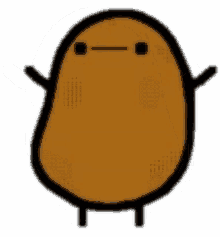
\includegraphics[width=0.75\linewidth]{patata}
    \caption{Patata para rellenar el espacio}
    \label{fig:patata}
\end{figure}
\newpage

\section{10/04 - Medidas de Dispersión}
\textbf{\textit{Objetivo: Aplicar y comprender propiedades de las medidas de dispersión}}
\subsection{Medidas de Dispersión}
Las medidas de tendencia central (como la media) no son suficientes por sí solas para describir un conjunto de datos, ya que no indican cuán dispersos o concentrados están los datos alrededor de ese centro. Consideremos dos conjuntos con la misma media $\bar{x}=0$:
\[ A = \{-4, 4, -4, 4\} \quad (\text{Media } \bar{x}_A = 0) \]
\[ B = \{7, 1, -6, -2\} \quad (\text{Media } \bar{x}_B = 0) \]
Ambos tienen $\bar{x}=0$, pero los datos en el conjunto $A$ están menos dispersos (más concentrados alrededor de la media) que en el conjunto $B$. Las medidas de dispersión cuantifican esta variabilidad o "esparcimiento" de los datos.

\subsubsection{Rango (o Amplitud Total):}
Se define como la diferencia entre el valor máximo y el valor mínimo de los datos.
\[ Rango = x_{max} - x_{min} \]
Es una medida simple pero muy sensible a valores extremos y no considera la distribución de los datos intermedios.

\subsubsection{Desviación Media (DM):}
Dada una variable $X$, con $n$ datos $x_1, x_2, \dots, x_n$ y media aritmética $\bar{x}$. Se define la desviación media como el promedio de las desviaciones absolutas de cada dato respecto a la media:
\[ DM = \frac{|x_1-\bar{x}|+|x_2-\bar{x}|+\dots+|x_n-\bar{x}|}{n} = \frac{\sum_{i=1}^{n} |x_i - \bar{x}|}{n} \]
Mide el promedio de cuánto se desvían los datos de la media, en valor absoluto.

\subsubsection{Varianza ($\sigma^2$ para población, $s^2$ para muestra):}
Es el promedio de las desviaciones al cuadrado de cada dato respecto a la media. Es la medida de dispersión más utilizada junto con su raíz cuadrada (la desviación estándar).
Para una \textbf{población} de $N$ datos:
\[ \sigma^2 = \frac{\sum_{i=1}^{N} (x_i - \mu)^2}{N} \]
Donde $\mu$ es la media poblacional. Si los datos $x_1, \dots, x_n$ constituyen toda la población (y $\bar{x}$ es su media):
\[ \sigma^2 = \frac{\sum_{i=1}^{n} (x_i - \bar{x})^2}{n} \]
Para una \textbf{muestra} de $n$ datos, la varianza muestral \textit{insesgada} (estimador de $\sigma^2$) es:
\[ s^2 = \frac{\sum_{i=1}^{n} (x_i - \bar{x})^2}{n-1} \]
(En este curso, si no se especifica, $\sigma^2$ con denominador $n$ se refiere a la varianza de un conjunto de datos específico, sea este una población o una muestra descripta como tal).

\subsubsection{Desviación Estándar (o Típica) ($\sigma$ para población, $s$ para muestra):}
Es la raíz cuadrada positiva de la varianza. Tiene la ventaja de estar expresada en las mismas unidades que los datos originales.
\[ \sigma = \sqrt{\sigma^2} = \sqrt{\frac{\sum_{i=1}^{n} (x_i - \bar{x})^2}{n}} \]
\[ s = \sqrt{s^2} = \sqrt{\frac{\sum_{i=1}^{n} (x_i - \bar{x})^2}{n-1}} \]

\subsubsection{Propiedades de $\sigma$ y $\sigma^2$ (usando la definición con denominador $n$)}
\begin{center}
    \begin{enumerate}
        \item $\sigma \ge 0$ y $\sigma^2 \ge 0$. Son siempre no negativas.
        \item $\sigma = 0 \iff \sigma^2 = 0 \iff x_i = \bar{x}$ para todo $i \iff x_i = x_j$ para todo $i, j \in \{1, \dots, n\}$. La desviación estándar (y varianza) es cero si y sólo si todos los datos son iguales.
        \item Si a todos los datos de un conjunto se les suma (o resta) una constante $k$ (transformación $y_i = x_i + k$), la nueva media es $\bar{y} = \bar{x} + k$, pero la varianza y la desviación estándar no cambian: $\sigma_y^2 = \sigma_x^2$ y $\sigma_y = \sigma_x$.
        \item Si todos los datos de un conjunto se multiplican (o dividen) por una constante $k$ (transformación $y_i = k \cdot x_i$), la nueva media es $\bar{y} = k\bar{x}$, la nueva varianza es $\sigma_y^2 = k^2 \sigma_x^2$, y la nueva desviación estándar es $\sigma_y = |k| \sigma_x$.
        \item Fórmula computacional (o abreviada) para la varianza: $\sigma^2 = \frac{\sum x_i^2}{n} - (\bar{x})^2 = \overline{x^2} - (\bar{x})^2$. Es decir, la varianza es la media de los cuadrados de los datos menos el cuadrado de la media de los datos.
        \item $\sigma^2=\sigma \iff \sigma=0 \vee \sigma=1$. (Asumiendo que $\sigma$ es el valor numérico de la desviación estándar).
        \item $\sigma^2 < \sigma \iff 0 < \sigma < 1$.
        \item $\sigma^2 > \sigma \iff \sigma > 1$.
    \end{enumerate}
\end{center}
\newpage

\section{16/04 - Propiedades de la Varianza y Desviación Estándar}
\subsection{Demostración Propiedad 4 (Multiplicación por una constante)}
Sea la variable $X$ con datos $x_1, \dots, x_n$, media $\bar{x}$ y varianza $\sigma_x^2$.
Sea $Y$ una nueva variable tal que $y_i = k \cdot x_i$ para cada $i$.
Sabemos que la media de $Y$ es $\bar{y} = k \cdot \bar{x}$.
La varianza de $Y$, $\sigma_y^2$, se define como:
\[\sigma_y^2=\frac{\sum_{i=1}^{n} (y_i - \bar{y})^2}{n} \]
Sustituyendo $y_i = kx_i$ y $\bar{y} = k\bar{x}$:
\[\sigma_y^2=\frac{\sum_{i=1}^{n} (kx_i - k\bar{x})^2}{n}\]
Factorizando $k$ dentro del paréntesis al cuadrado:
\[\sigma_y^2=\frac{\sum_{i=1}^{n} [k(x_i - \bar{x})]^2}{n}\]
Aplicando la potencia al producto:
\[\sigma_y^2=\frac{\sum_{i=1}^{n} k^2(x_i - \bar{x})^2}{n}\]
Como $k^2$ es una constante para la sumatoria, puede salir fuera:
\[\sigma_y^2=k^2 \cdot \frac{\sum_{i=1}^{n} (x_i - \bar{x})^2}{n}\]
Reconociendo que $\frac{\sum_{i=1}^{n} (x_i - \bar{x})^2}{n}$ es la definición de $\sigma_x^2$:
\[\sigma_y^2=k^2 \cdot \sigma_x^2\]
Tomando la raíz cuadrada positiva para obtener la desviación estándar (ya que $\sigma_x \ge 0$):
\[\sigma_y = \sqrt{k^2 \cdot \sigma_x^2} = \sqrt{k^2} \cdot \sqrt{\sigma_x^2} = |k| \cdot \sigma_x\]
L.Q.Q.D. (Lo Que Queríamos Demostrar)

\subsection{Ejercicio}
Dados los datos: -2, 0, 2, 4, 6. ($n=5$). Determinar:
\begin{enumerate}
    \item $\bar{x}$ \\
        \textit{Solución:} $\bar{x} = \frac{-2+0+2+4+6}{5} = \frac{10}{5} = 2$. \\
    \item $\sigma$ (desviación estándar) \\
        \textit{Solución:} Primero calculamos la varianza $\sigma^2$:
        \begin{align*} \sigma^2 &= \frac{\sum (x_i - \bar{x})^2}{n} \\ &= \frac{(-2-2)^2+(0-2)^2+(2-2)^2+(4-2)^2+(6-2)^2}{5} \\ &= \frac{(-4)^2+(-2)^2+(0)^2+(2)^2+(4)^2}{5} \\ &= \frac{16+4+0+4+16}{5} = \frac{40}{5} = 8 \end{align*}
        Ahora la desviación estándar: $\sigma = \sqrt{\sigma^2} = \sqrt{8} = \sqrt{4 \cdot 2} = 2\sqrt{2} \approx 2.828$. \\
    \item $\overline{x^2}$ (el promedio de los cuadrados de los datos) \\
        \textit{Solución:} Los cuadrados de los datos son: $(-2)^2=4, 0^2=0, 2^2=4, 4^2=16, 6^2=36$.
        \[ \overline{x^2} = \frac{4+0+4+16+36}{5} = \frac{60}{5} = 12 \]
    \item Calcular $\overline{x^2}-(\bar{x})^2$ y comparar con $\sigma^2$. \\
        \textit{Solución:} $\overline{x^2}-(\bar{x})^2 = 12 - (2)^2 = 12 - 4 = 8$. \\
        Este resultado (8) es igual a la varianza $\sigma^2$ calculada en el punto 2, lo cual verifica la propiedad 5 (fórmula computacional de la varianza).
\end{enumerate}
\newpage

\subsection{Demostración Propiedad 5 (Fórmula Computacional de la Varianza)}
Partimos de la definición de varianza (usando denominador $n$):
\[\sigma^2=\frac{\sum_{i=1}^{n} (x_i-\bar{x})^2}{n}\]
Expandimos el binomio al cuadrado $(a-b)^2 = a^2 - 2ab + b^2$:
\[\sigma^2=\frac{\sum_{i=1}^{n} (x_i^2 - 2x_i\bar{x} + (\bar{x})^2)}{n}\]
Distribuimos la sumatoria y el denominador $n$:
\[\sigma^2=\frac{\sum x_i^2}{n} - \frac{\sum 2x_i\bar{x}}{n} + \frac{\sum (\bar{x})^2}{n}\]
En el segundo término, $2\bar{x}$ es una constante respecto a la suma $\sum x_i$. En el tercer término, $(\bar{x})^2$ es una constante, y $\sum_{i=1}^{n} (\bar{x})^2 = n(\bar{x})^2$.
\[\sigma^2=\frac{\sum x_i^2}{n} - 2\bar{x} \frac{\sum x_i}{n} + \frac{n(\bar{x})^2}{n}\]
Reconocemos que $\frac{\sum x_i^2}{n} = \overline{x^2}$ (la media de los cuadrados) y $\frac{\sum x_i}{n} = \bar{x}$ (la media):
\[\sigma^2=\overline{x^2} - 2\bar{x} (\bar{x}) + (\bar{x})^2\]
\[\sigma^2=\overline{x^2} - 2(\bar{x})^2 + (\bar{x})^2\]
\[\sigma^2=\overline{x^2} - (\bar{x})^2\]
L.Q.Q.D.
\newpage

    \section{23/04 - Demostraciones sobre el Valor de la Desviación Estándar}
        \subsection{Demostraciones de Propiedades Relacionadas con el Valor de $\sigma$}
            Recordar que $\sigma \ge 0$ por definición (es una raíz cuadrada positiva o cero).

            \subsubsection{Propiedad 6: $\sigma^2 = \sigma \iff \sigma=0 \vee \sigma=1$}
                Partimos de la ecuación:
                \[\sigma^2=\sigma \]
                Reordenamos para formar una ecuación cuadrática en $\sigma$:
                \[\sigma^2-\sigma=0 \]
                Factorizamos $\sigma$:
                \[\sigma(\sigma-1)=0 \]
                Esto implica que uno de los factores debe ser cero:
                \[\sigma=0 \quad \text{o} \quad \sigma-1=0 \]
                Por lo tanto:
                \[\sigma=0 \vee \sigma=1 \]
                L.Q.Q.D.

            \subsubsection{Propiedad 7: $\sigma^2 < \sigma \iff 0 < \sigma < 1$}
                Partimos de la desigualdad:
                \[\sigma^2 < \sigma \]
                Reordenamos:
                \[\sigma^2-\sigma < 0 \]
                Factorizamos:
                \[\sigma(\sigma-1) < 0 \]
                Para que el producto de dos factores sea negativo, uno debe ser positivo y el otro negativo. Analizamos los signos de $\sigma$ y $(\sigma-1)$:
                
                \begin{center}
                    \begin{tabular}{c|ccccc}
                        Intervalo & $(-\infty, 0)$ & $0$ & $(0, 1)$ & $1$ & $(1, +\infty)$ \\
                        \hline
                        Signo de $\sigma$ & $-$ & $0$ & $+$ & $+$ & $+$ \\
                        Signo de $(\sigma-1)$ & $-$ & $-$ & $-$ & $0$ & $+$ \\
                        \hline
                        Signo de $\sigma(\sigma-1)$ & $+$ & $0$ & $-$ & $0$ & $+$ \\
                    \end{tabular}
                \end{center}
                
                La desigualdad $\sigma(\sigma-1) < 0$ se cumple cuando $\sigma \in (0, 1)$.
                Dado que $\sigma \ge 0$ por definición, el intervalo $(-\infty, 0)$ no es relevante para la desviación estándar.
                Por lo tanto:
                \[0 < \sigma < 1 \]
                L.Q.Q.D.

            \subsubsection{Propiedad 8: $\sigma^2 > \sigma \iff \sigma > 1$}
                Partimos de la desigualdad:
                \[\sigma^2 > \sigma \]
                Reordenamos:
                \[\sigma^2-\sigma > 0 \]
                Factorizamos:
                \[\sigma(\sigma-1) > 0 \]
                Para que el producto de dos factores sea positivo, ambos deben ser positivos o ambos deben ser negativos. Usando la tabla de signos anterior:
                \begin{itemize}
                    \item Ambos negativos: $\sigma < 0$ y $\sigma-1 < 0$ (es decir, $\sigma < 0$). No es posible para $\sigma$.
                    \item Ambos positivos: $\sigma > 0$ y $\sigma-1 > 0$ (es decir, $\sigma > 1$).
                \end{itemize}
                La desigualdad $\sigma(\sigma-1) > 0$ se cumple cuando $\sigma \in (-\infty, 0) \cup (1, +\infty)$.
                Considerando la restricción $\sigma \ge 0$:
                \begin{itemize}
                    \item Si $\sigma=0$, entonces $\sigma(\sigma-1)=0$, lo cual no satisface $0>0$.
                    \item El intervalo $(-\infty,0)$ no es válido para $\sigma$.
                    \item Nos queda el intervalo $(1, +\infty)$.
                \end{itemize}
                Por lo tanto:
                \[\sigma > 1\]
                L.Q.Q.D.
                \newpage



\section{30/05 - Medidas de Posición: Cuartiles, Quintiles, Deciles y Percentiles}
Dado un Conjunto de datos Ordenados se define:

\subsection{Cuartiles}
Son tres valores que dividen en parte iguales a un conjuntode datos ordenaods. Se denominan $Q_1$, $Q_2$ y $Q_3$
\textbf{Observacion:} $Q_2 = Me$

\subsection{Quintiles}
Son los 4 valores que dividen en partes igaules a los datos, que corresponden al 20\%, 40\%, 60\% y 80\%

\subsection{Deciles}
Son los 9 valores que dividen en partes igaules a los datos, que corresponden al 10\%, 20\%, 30\%, 40\%, 50\%, 60\%, 70\%, 80\% y 90\%


\subsection{Percentiles}
Son los 99 valores que dividen en partes igaules a los datos, que corresponden al 1\%, 2\%, 3\%, ... ,99\%
\[ P_i= \frac{i \cdot n}{100} \] Corresponde a la posición del percentil.


\newpage

\section{11/06 - Principios Fundamentales de la Combinatoria}
\subsection{Combinatoria} 
Son técnicas de conteo. Sean A y B dos sucesos, que pueden ocurrir de $a$ y $b$ maneras respectivamente.
\begin{itemize}
    \item \textbf{\textit{Principio Aditivo:}} Si los sucesos no pueden ocurrir de manera simultánea (son mutuamente excluyentes), entonces hay \textit{a+b} maneras posibles de que ocurra \textit{A o B}.
    \item \textbf{\textit{Principio Multiplicativo:}} Si los sucesos ocurren uno a continuación del otro o de manera simultánea, entonces hay $a \cdot b$ formas de que ocurra \textit{A y B}.
\end{itemize}

\subsection{Ejercicios}
\begin{enumerate}
    \item Al lanzar una moneda y un dado, ¿cuántos resultados posibles hay? \\
    \textit{Solución:}
    Lanzar una moneda y un dado son sucesos independientes que ocurren simultáneamente. Usamos el principio multiplicativo.
    \begin{itemize}
        \item Resultados de la moneda: 2 (cara, sello).
        \item Resultados del dado: 6 (1, 2, 3, 4, 5, 6).
    \end{itemize}
    Total de resultados: $2 \times 6 = 12$. \\
    \textbf{Respuesta: 12 resultados posibles.}

    \item Si Pedro tiene 5 lápices de pasta, 4 de tinta y 3 de grafito, ¿de cuántas maneras puede elegir un lápiz para escribir? \\
    \textit{Solución:}
    Pedro debe elegir un lápiz de pasta \textbf{o} uno de tinta \textbf{o} uno de grafito. Son elecciones mutuamente excluyentes. Usamos el principio aditivo.
    \begin{itemize}
        \item Maneras de elegir un lápiz de pasta: 5.
        \item Maneras de elegir un lápiz de tinta: 4.
        \item Maneras de elegir un lápiz de grafito: 3.
    \end{itemize}
    Total de maneras: $5 + 4 + 3 = 12$. \\
    \textbf{Respuesta: 12 maneras distintas.}

    \item En un local se puede elegir un combo con las siguientes opciones disponibles: 5 tipos de hamburguesas, 4 bebidas distintas o bien un jugo de 2 sabores distintos. Si el combo consiste en una hamburguesa y una bebida/jugo, ¿de cuántas maneras distintas se puede elegir? \\
    \textit{Solución:}
    La elección del combo tiene dos etapas: elegir una hamburguesa \textbf{y} elegir un líquido.
    \begin{itemize}
        \item \textbf{Etapa 1 (Hamburguesa):} Hay 5 opciones.
        \item \textbf{Etapa 2 (Líquido):} Se puede elegir una bebida \textbf{o} un jugo. Esta es una sub-decisión que usa el principio aditivo.
        \begin{itemize}
            \item Opciones de bebida: 4.
            \item Opciones de jugo: 2.
            \item Total de opciones de líquido: $4 + 2 = 6$.
        \end{itemize}
    \end{itemize}
    Para formar el combo, se aplica el principio multiplicativo entre la Etapa 1 y la Etapa 2.
    Total de combos: $5 \text{ (hamburguesas)} \times 6 \text{ (líquidos)} = 30$. \\
    \textbf{Respuesta: Se puede elegir de 30 maneras distintas.}
\end{enumerate}
\newpage


\section{07/07 - Permutaciones}
\textbf{\textit{\large{Diferenciar distintas Permutaciones}}}

\subsection{Combinatoria}
Evento A: a maneras 

Evento B: b maneras

\begin{itemize}
    \item Principio Aditivo: $a + b$ \textbf{Excluyentes}
    \item Principio Multiplicativo: $a \cdot b$ \textbf{Simultaneos} 
    \item \textbf{\textit{Ej:}}
    \begin{itemize}
        \item Evento A: Lamzar un dado
        \item Evento B: lanzar un dado 2 veces
    \end{itemize}
\end{itemize}

\subsubsection{Permutacion simple} Correpsonde a la manera en que se pueden ordenar $n$ objetos

    \begin{minipage}{0.35\textwidth}
        \centering
        \[ P_n = n! \]
    \end{minipage}
    \hfill
    \begin{minipage}{0.55\textwidth}
        \centering
        \[ P_4 = 4!= 4 \cdot 3 \cdot 2 \cdot 1 \]
    \end{minipage}

\subsubsection{Permutacion con repetición} Si tienes $n$ elementos y un elemento se repite $r_1$ veces, otro $r_2$ veces y así sucesivamente, entonces se pueden ordenar:

\[ P_{r_1, r_2, ...}^n = \frac{n!}{r_1! \cdot r_2! \cdot ...} \]


\subsubsection{Permutacion Circular} Si tenemos $n$ elementos, los podemos ordenar de :
\[ PC_n = \frac{n!}{n} = (n-1)! \]

\subsection{Ejercicios}

\begin{enumerate}[label=\alph*.)]
    \item ¿De cuantas maneras se peuden ordenar las letras de la palabara LEMUR  para fomrar otra palabara (con o sin sentido)
        \[ P_5 = 5! = 5 \cdot 4 \cdot 3 \cdot 2 \cdot 1 = 120 \] \\

    \item ¿Y para la plabra ARROYO? ¿Y CARRERA?

        \begin{minipage}{0.45\textwidth}
            \centering
            \textbf{ARROYO:}
            \[ P_{2, 2}^6 = \frac{6!}{2! \cdot 2!} = \frac{720}{4} = 180 \]
        \end{minipage}
        \hfill
        \begin{minipage}{0.45\textwidth}
            \centering
            \textbf{CARRERA}
            \[ P_{2,3}^7 = \frac{7!}{2! \cdot 3!} = \frac{7\cdot 6 \cdot 5 \cdot 4}{2} = 420 \]
        \end{minipage}
        
        \phantom p \\

    \item ¿De cuantas maneras se pueden sentar en una mesa de 4 sillas, 4 personas?
        \[ PC_4 = \frac{4!}{4} =\frac{4 \cdot 3!}{4} = 3! = 6 \]
\end{enumerate}
\newpage

\section{04/08 - Variaciones y Combinaciones}
    \subsection{Variacion(o arreglo)}
        Corres al número de ordenaciones de $K$ elementos, con $k \leq n$, de un total de $n$ elementos.
        \[V_k^n = n \cdot (n - 1) \cdot (n - 2) \cdot ... \cdot (n - (k - 1)) = \frac{n!}{(n - k)!} \]
        \subsubsection*{Con repetición}
            \[VR_k^n = n^k \]
    \subsection{Combinaciones} Corresponde a la cantiadad de grupos (o subconjuntos) de $k$ ekemnots de un total de n elemntos. 
        \[C_k^n = \frac{V_k^n}{k!} = \frac{n!}{(n - k)! \cdot k!} \]

    \subsection*{¿Cómo Diferenciar?}
Para determinar qué fórmula usar, sigue este diagrama de flujo:

% CORREGIDO: Se reestructuró la lista para evitar el error "Too deeply nested".
% Se simplificaron las opciones de 'enumerate'.
\begin{enumerate}[label=\bfseries Paso \arabic*:, wide]
    \item \textbf{¿Importa el orden de los elementos seleccionados?}
    \begin{itemize}
        \item[\bfseries a)] \textbf{Sí, el orden importa $\rightarrow$ PERMUTACIÓN / VARIACIÓN}
            \begin{itemize}
                \item \textbf{¿Se usan TODOS los elementos ($k=n$)? $\rightarrow$ PERMUTACIÓN}
                    \begin{itemize}
                        \item ¿Hay elementos repetidos? (ej. palabra C-A-S-A) $\rightarrow$ Permutación con repetición: $P_{n_1, \dots, n_k}^n = \frac{n!}{n_1! \dots n_k!}$
                        \item ¿Son todos los elementos distintos? $\rightarrow$ Permutación simple: $P_n = n!$
                    \end{itemize}
                \item \textbf{¿Se elige un SUBCONJUNTO ($k<n$)? $\rightarrow$ VARIACIÓN}
                    \begin{itemize}
                        \item ¿Se permite repetir elementos? $\rightarrow$ Variación con repetición: $VR_k^n = n^k$
                        \item ¿No se permite repetir? $\rightarrow$ Variación simple: $V_k^n = \frac{n!}{(n-k)!}$
                    \end{itemize}
            \end{itemize}
        \item[\bfseries b)] \textbf{No, el orden NO importa $\rightarrow$ COMBINACIÓN}
            \begin{itemize}
                \item ¿Se permite repetir elementos? $\rightarrow$ Combinación con repetición: $CR_k^n = \binom{n+k-1}{k}$
                \item ¿No se permite repetir? $\rightarrow$ Combinación simple: $C_k^n = \binom{n}{k} = \frac{n!}{k!(n-k)!}$
            \end{itemize}
    \end{itemize}
\end{enumerate}

\subsection*{Ejercicios Resueltos}
Aquí tienes los ejercicios con sus soluciones y el razonamiento para cada uno:

\begin{enumerate}[leftmargin=*,label=\arabic*.]
    \item \textbf{En una carrera participan 15 estudiantes. ¿De cuantas maneras se puede formar el podio (1er, 2do, 3er lugar)?}
    \begin{itemize}
        \item \textbf{Razonamiento:} El orden importa (1er lugar es diferente de 2do). No hay repetición de estudiantes. Se seleccionan 3 de 15. Esto es una **Variación simple**.
        \item \textbf{Cálculo:} $V_3^{15} = 15 \cdot 14 \cdot 13 = 2730$ maneras.
    \end{itemize}

    \item \textbf{¿De cuantas maneras se puede formar una clave numérica de 4 dígitos?}
    \begin{itemize}
        \item \textbf{Razonamiento:} El orden importa (1234 es diferente de 4321). Los dígitos pueden repetirse (ej. 1111). Se seleccionan 4 dígitos de 10 posibles (0-9). Esto es una **Variación con repetición**.
        \item \textbf{Cálculo:} $VR_4^{10} = 10^4 = 10000$ maneras.
    \end{itemize}

    \item \textbf{¿Y si no se repiten los dígitos (para la clave numérica de 4 dígitos)?}
    \begin{itemize}
        \item \textbf{Razonamiento:} El orden sigue importando. Los dígitos NO pueden repetirse. Se seleccionan 4 dígitos distintos de 10 posibles. Esto es una **Variación simple**.
        \item \textbf{Cálculo:} $V_4^{10} = 10 \cdot 9 \cdot 8 \cdot 7 = 5040$ maneras.
    \end{itemize}

    \item \textbf{En un curso de 40 estudiantes, ¿Cuántas directivas (Presidente, Vicepresidente, Tesorero) se pueden formar?}
    \begin{itemize}
        \item \textbf{Razonamiento:} El orden importa (ser Presidente es distinto de ser Vicepresidente). Los estudiantes no pueden ocupar múltiples cargos. Se seleccionan 3 de 40. Esto es una **Variación simple**.
        \item \textbf{Cálculo:} $V_3^{40} = 40 \cdot 39 \cdot 38 = 59280$ maneras.
    \end{itemize}

    \item \textbf{En una asamblea de 100 personas, se escoge una directiva de 3 personas ¿De cuantas maneras se puede hacer?}
    \begin{itemize}
        \item \textbf{Razonamiento:} Esta pregunta es ambigua. Si "directiva" implica roles específicos (similar al ejercicio anterior), el orden importa. Sin embargo, si es solo un grupo de 3 personas sin roles definidos, el orden no importa (ver el siguiente ejercicio). Asumiendo que se refiere a un grupo donde el orden no importa, como una comisión.
        \item \textbf{Cálculo (asumiendo que el orden NO importa, es decir, una comisión):} $C_3^{100} = \frac{100 \cdot 99 \cdot 98}{3 \cdot 2 \cdot 1} = \frac{970200}{6} = 161700$ maneras.
        \item \textbf{Nota:} Si la intención era que el orden SÍ importaba (ej. Presidente, Secretario, Vocal), entonces sería una Variación: $V_3^{100} = 100 \cdot 99 \cdot 98 = 970200$ maneras. Es crucial aclarar si los roles son distinguibles o no en el enunciado.
    \end{itemize}

    \item \textbf{Y cuantas comisiones de 3 personas se pueden hacer (en la asamblea de 100 personas)?}
    \begin{itemize}
        \item \textbf{Razonamiento:} El orden NO importa (una comisión de Juan, Pedro y María es la misma que María, Pedro y Juan). No hay repetición de personas. Se seleccionan 3 de 100. Esto es una **Combinación simple**.
        \item \textbf{Cálculo:} $C_3^{100} = \frac{100!}{3!(100-3)!} = \frac{100 \cdot 99 \cdot 98}{3 \cdot 2 \cdot 1} = \frac{970200}{6} = 161700$ maneras.
    \end{itemize}
\end{enumerate}

\newpage

\section{11/08 - Propiedades de Combinatoria y Triángulo de Pascal}
\subsection{Propiedades de los Números Combinatorios}
Los números combinatorios, denotados como $\binom{n}{k}$, tienen propiedades útiles que simplifican los cálculos. [1]
\begin{enumerate}
    \item \textbf{Combinaciones de los extremos:} Seleccionar todos los elementos de un conjunto es posible de una sola manera, al igual que no seleccionar ninguno (eligiendo el conjunto vacío).
    \[ \binom{n}{n} = \binom{n}{0} = 1 \]

    \item \textbf{Propiedad de simetría:} El número de maneras de elegir $k$ elementos de un conjunto de $n$ es igual al número de maneras de *no elegir* (o dejar) $n-k$ elementos.
    \[ \binom{n}{k} = \binom{n}{n-k} \quad \text{para } k \leq n \]

    \item \textbf{Identidad de Pascal:} Esta identidad es la base para construir el Triángulo de Pascal. [2] Establece que la suma de dos números combinatorios consecutivos en una fila del triángulo da como resultado el número combinatorio que se encuentra debajo de ellos.
    \[ \binom{n}{k} + \binom{n}{k+1} = \binom{n+1}{k+1} \]
\end{enumerate}

\subsection{Demostraciones}
La demostración se basa en la aplicación directa de la fórmula de la combinación, $\binom{n}{k} = \frac{n!}{k!(n-k)!}$, y en la definición matemática de que $0! = 1$.

\vspace{1em}
\noindent \textbf{Caso 1: $\binom{n}{n}$}
\[ \binom{n}{n} = \frac{n!}{(n-n)! \cdot n!} = \frac{n!}{0! \cdot n!} \]
\textit{Comentario: Al aplicar la fórmula, el término $(n-n)!$ se convierte en $0!$. Luego, los términos $n!$ del numerador y denominador se cancelan, dejando $1/0!$. Como $0!$ es 1, el resultado es 1.}
\[ \frac{n!}{0! \cdot n!} = \frac{1}{0!} = \frac{1}{1} = 1 \]
\textit{Interpretación: Solo hay una forma de elegir n elementos de un conjunto de n (es decir, tomarlos todos).}

\vspace{1em}
\noindent \textbf{Caso 2: $\binom{n}{0}$}
\[ \binom{n}{0} = \frac{n!}{(n-0)! \cdot 0!} = \frac{n!}{n! \cdot 0!} \]
\textit{Comentario: De forma similar, $(n-0)!$ es simplemente $n!$. Al cancelar los términos $n!$, nuevamente obtenemos $1/0!$, que es igual a 1.}
\[ \frac{n!}{n! \cdot 0!} = \frac{1}{0!} = \frac{1}{1} = 1 \]
\textit{Interpretación: Solo hay una forma de elegir 0 elementos de un conjunto (es decir, no tomar ninguno).}

\subsubsection{Propiedad 2 (Simetría): $\binom{n}{k} = \binom{n}{n-k}$}
\textit{Comentario: Esta propiedad muestra una hermosa simetría en las combinaciones. Intuitivamente, significa que el acto de elegir $k$ elementos para formar un grupo es equivalente al acto de elegir $n-k$ elementos para dejarlos fuera de ese grupo. La demostración es algebraica.}

\vspace{1em}
\noindent Partimos de la definición de $\binom{n}{k}$:
\[ \binom{n}{k} = \frac{n!}{k! \cdot (n-k)!} \]
\textit{Comentario: El producto en el denominador es conmutativo, lo que significa que podemos cambiar el orden de $k!$ y $(n-k)!$ sin alterar el resultado.}
\[ \frac{n!}{k! \cdot (n-k)!} = \frac{n!}{(n-k)! \cdot k!} \]
\textit{Comentario: Ahora, si observamos esta expresión final, corresponde exactamente a la definición de $\binom{n}{n-k}$. Por lo tanto, hemos demostrado que las dos expresiones son iguales.}
\[ \binom{n}{n-k} = \frac{n!}{(n-k)! \cdot (n-(n-k))!} = \frac{n!}{(n-k)! \cdot k!} \]
Así, se concluye que $\binom{n}{k} = \binom{n}{n-k}$.

\subsection{Triángulo de Pascal y Binomio de Newton}
El \textbf{Triángulo de Pascal} es una disposición triangular de números donde cada número es la suma de los dos que tiene directamente encima. [9] Este triángulo está íntimamente relacionado con el \textbf{Teorema del Binomio} (o Binomio de Newton), que proporciona una fórmula para expandir potencias de un binomio $(a+b)^n$.

La fórmula del Binomio de Newton utiliza los números combinatorios como coeficientes para cada término de la expansión. [9, 10] Notablemente, los coeficientes de la expansión de $(a+b)^n$ corresponden exactamente a los números en la fila $n+1$ del Triángulo de Pascal.
\[ (a+b)^n = \sum_{k=0}^{n} \binom{n}{k} a^{n-k} b^k = \binom{n}{0}a^n + \binom{n}{1}a^{n-1}b + \dots + \binom{n}{n}b^n \]

\begin{figure}[h!]
    \centering
    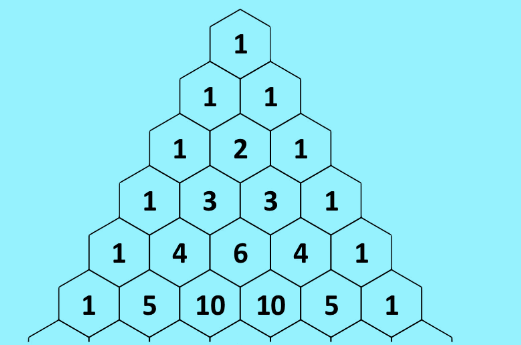
\includegraphics[width=0.5\textwidth]{pascal}
    \caption{El Triángulo de Pascal, donde cada fila $n$ corresponde a los coeficientes de $(a+b)^n$.}
    \label{fig:pascaltrig}
\end{figure}


\subsection{Conjunto Potencia}
El \textbf{Conjunto Potencia} de un conjunto $A$, denotado como $P(A)$, es el conjunto formado por \textbf{todos los subconjuntos} posibles de $A$, incluyendo el conjunto vacío y el propio conjunto $A$. [12, 14]

La \textbf{cardinalidad} (número de elementos) del conjunto potencia se puede calcular sumando el número de subconjuntos de cada tamaño posible (de tamaño 0, de tamaño 1, de tamaño 2, etc.), lo cual es una suma de números combinatorios. Si el conjunto original $A$ tiene $n$ elementos, la cardinalidad de su conjunto potencia es $2^n$. [3, 6]
\[ |P(A)| = \sum_{k=0}^{n} \binom{n}{k} = 2^n \]

\subsection{Ejercicios}
\begin{enumerate}
    \item \textbf{¿De cuántas maneras se pueden sentar 5 personas en una mesa redonda?} \\
    \textit{Solución:} Es una permutación circular. $PC_5 = (5-1)! = 4! = 24$ maneras.

    \item \textbf{En una competición participan 40 personas y solo quedan seleccionadas 5.}
        \begin{enumerate}
            \item \textbf{¿Cuántos grupos distintos pueden quedar seleccionados?} \\
            \textit{Solución:} El orden no importa, es una combinación. \\
            $C_5^{40} = \binom{40}{5} = \frac{40!}{5!(35!)} = \frac{40 \cdot 39 \cdot 38 \cdot 37 \cdot 36}{5 \cdot 4 \cdot 3 \cdot 2 \cdot 1} = 658,008$ grupos.
            \item \textbf{¿Cuántos primeros 5 puntajes distintos puede haber?} \\
            \textit{Solución:} El orden importa (1er, 2do, etc.), es una variación. \\
            $V_5^{40} = \frac{40!}{(40-5)!} = \frac{40!}{35!} = 40 \cdot 39 \cdot 38 \cdot 37 \cdot 36 = 78,960,960$ maneras.
        \end{enumerate}

    \item \textbf{Si se dispone de 5 frutas distintas.}
        \begin{enumerate}
            \item \textbf{¿Cuántos jugos de dos frutas se pueden hacer?} \\
            \textit{Solución:} El orden no importa, es una combinación. \\
            $C_2^5 = \binom{5}{2} = \frac{5!}{2!3!} = 10$ jugos.
            \item \textbf{¿Y de 3 frutas?} \\
            \textit{Solución:} Combinación. $C_3^5 = \binom{5}{3} = \frac{5!}{3!2!} = 10$ jugos.
            \item \textbf{¿Y de al menos 2 frutas?} \\
            \textit{Solución:} Se suman los jugos de 2, 3, 4 y 5 frutas. \\
            $C_2^5 + C_3^5 + C_4^5 + C_5^5 = 10 + 10 + 5 + 1 = 26$ jugos.
        \end{enumerate}
\end{enumerate}
\begin{figure}[h!]
    \centering
    
\includegraphics[width=0.75\textwidth]{Gat}
    \caption{Gatito Para hacer bonito el apunte}
    \label{fig:Gat}
\end{figure}


\newpage

\end{document}
